\documentclass[resume]{subfiles}


\begin{document}
\section{Observabilité}
\subsection{Définition}

Le système $\dot{x}(t) = Ax (t)$, $y = Cx(t)$   est complètement observable s'il existe un temps fini $t^* > 0$ tel que la  connaissance de $y (t)$  sur $[0\space t^*]$est suffisante pour déterminer la valeur de l'état initial $x(0)$

\subsection{Théorème}

Un système à temps continu (discret) est complètement observable si et  seulement si la matrice d'observabilité: $S^T = [C, CA, CA^2 ,..., CA^{n-1}]^T = [C^T, A^TC^T , (A^2)^T C^T,..., (A^{n-1})^T C^T]$ 

 est de rang n (rang plein)

\subsection{Observateur}

Un observateur est un système dynamique qui retourne une estimation de la valeur de l'état quand on le 'nourrit' avec les sorties mesurées.

\subsubsection{Observateur trivial (copie)}

Pour un système $\dot{x}(t)=Ax(t)+Bu(t)$

L'observateur est $\dot{z}(t)= Az(t)+Bu(t)$

Mais avec cette observateur l'erreur $\varepsilon(t)=z(t)-x(t)$ donc $\dot{\varepsilon}(t)=A\varepsilon(t)$ l'erreur disparait que lorsque le système est stable.

\subsubsection{Observateur identité}

Pour un système \begin{equation}\begin{cases}\dot{x}(t)=Ax(t)+Bu(t)\\y(t)=Cx(t)\end{cases}\end{equation} avec u et y connu

L'observateur est $\dot{z}(t)= Az(t)+E[y(t)-Cz(t)]+Bu(t)$ ou E est à choix

La dynamique de l'erreur est $\dot{\varepsilon}(t) = \dot{z}(t) - \dot{x}(t) = [A - EC] (z(t) - x(t)) = [A - EC] \varepsilon(t)$ 
\begin{itemize}
\item Si $z(0)=x(0)$ alors $z(t)=x(t)$ pour tout $t>0$ 
\item Si $z(0)\neq x(0)$ le vecteur d'erreur est gouverné par $[A-EC]$ 
\item On peut placer les valeurs propres de cette matrice, avec le degré de liberté que constitue E  
\end{itemize}
$A-EC$ donne la dynamique de l'observateur (qu'on va utiliser pour faire un placement de pôle de l'observateur). Attention ! La fonction place ou acker va déterminer $K$ dans $A-BK$. On doit donc faire
\verb!acker(A.T, C.T).T! (voir \ref{transpose_matrice})
\subsubsection{Observateur d'ordre réduit}

Un observateur d’ordre réduit peut être construit, pour que l'effort soit sur les variables "inconnues"

  Pour un système \begin{equation}\begin{cases}\dot{x}(t)=Ax(t)+Bu(t)\\y(t)=Cx(t)\end{cases}\end{equation} avec (A, C) complètement observable et C(pxn) de rang p

Voir les pages 14-16 du polycopier 2\_11 Observability 

\subsection{Contrôleur stabilisant}

\begin{figure}[H]
    \centering
    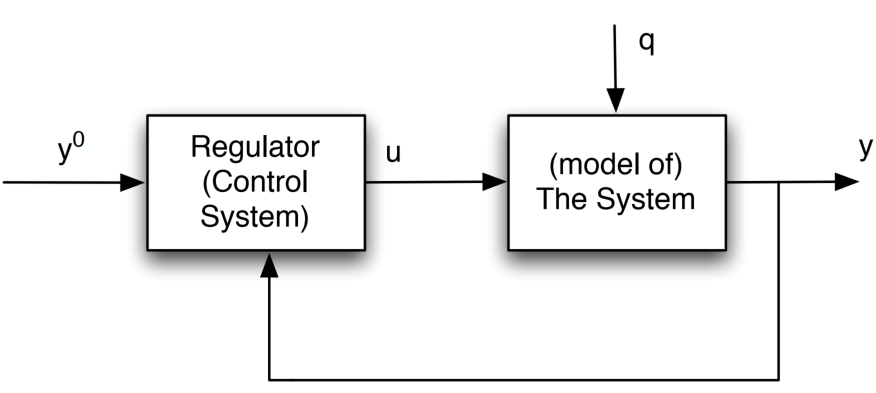
\includegraphics[width=1\columnwidth]{Figures/CtrlStab_1.png}
\end{figure}

\begin{figure}[H]
    \centering
    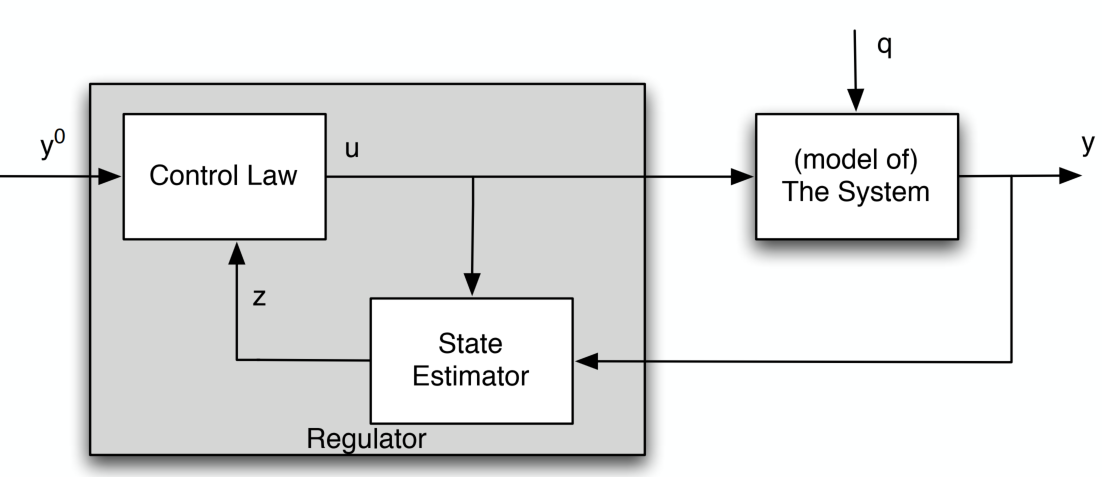
\includegraphics[width=1\columnwidth]{Figures/CtrlStab_2.png}
\end{figure}

\subsubsection{Théorème}

 Pour un système \begin{equation}\begin{cases}\dot{x}(t)=Ax(t)+Bu(t)\\y(t)=Cx(t)\end{cases}\end{equation} avec l'observateur identité $\dot{z}(t)= Az(t)+E[y(t)-Cz(t)]+Bu(t)$ et la loi de commande $u(t)=Kz(t)$ 

Le polynôme caractéristique de ce composite est égal au produit des
polynômes caractéristiques de $A+BK$ et de $A-EC$:  

$\Delta_{A+BK}(\lambda)\cdot \Delta_{A-EC}(\lambda)$  
\begin{itemize}
\item Les matrices $K$ et $E$ peuvent être fixées indépendamment
\item Ce théorème s'applique aux systèmes linéaires  
\end{itemize}

\end{document}